\chapter{Сравнение метода реконструкции освещения с аналогом}
\label{chap:light-comparison}

В данной главе приведены результаты испытаний метода реконструкции источников освещения, описанного в главе~5: точность реконструкции источников с гониометрической диаграммой направленности, время вычисления градиента и сравнение времени реконструкции с аналогом, выбранным по результатам обзора, --- системой дифференцируемого рендеринга Mitsuba~3~\cite{Mitsuba3} с методом path replay backpropagation (PRB)~\cite{PRB2021}.

\section{Условия проведения экспериментов}

Все эксперименты проводились на центральном процессоре AMD Ryzen~9 7950X (16 ядер, 32 потока) и графическом процессоре NVIDIA GeForce RTX~4090. Предложенный метод выполняется на центральном процессоре; графический процессор использовался только аналогом.

Сцена соответствует постановке задачи главы~5: пол и две стены, образующие угол, с серым ламбертовским материалом (альбедо 0.5); источник расположен над полом и направлен вниз. Используется одна камера, источник находится в поле её зрения. Разрешение входного изображения во всех экспериментах равно $1024\times1024$, глубина трассировки путей --- 6, то есть учитывается до пяти диффузных переотражений.

Точность оценивается по метрике PSNR между двумя изображениями одной сцены: эталонным и рассчитанным с восстановленным источником. Оба изображения переводятся в представление с ограниченным динамическим диапазоном одним и тем же преобразованием: умножением на общую экспозицию, при которой среднее значение эталона равно 0.5, кодированием по кривой sRGB и ограничением диапазоном $[0,1]$. Дополнительно приводится PSNR в линейном HDR-представлении, где пиковым значением считается максимум эталона.

\section{Точность реконструкции источников с гониометрической диаграммой}

Для проверки точности использовались восемь сцен с источниками трёх типов: точечным, диском и прямоугольником. Диаграммы направленности взяты из фотометрических файлов IES, входящих в набор тестов системы Hydra (тесты 206, 207, 208, 228, 232); среди них есть осесимметричные диаграммы с кольцевой структурой и несимметричные многолепестковые диаграммы. Цвет источника в части сцен отличается от белого.

Эталонное изображение рассчитывалось системой Hydra методом трассировки путей с многократной выборкой по значимости, 2048 лучей на пиксель. По этому изображению восстанавливались гониометрическая таблица разрешения $128\times64$ и цвет источника: 400 шагов метода Adam на четырёх уровнях разрешения таблицы, кэш световых путей с 16 лучами на пиксель. Затем сцена с восстановленным источником заново рассчитывалась системой Hydra с теми же настройками, что и эталон, и вычислялся PSNR между двумя изображениями. Таким образом, приведённая точность включает все погрешности метода, в том числе шум кэша и экспорт результата в файл IES.

\begin{table}[htbp]
    \centering
    \small
    \setlength{\tabcolsep}{4pt}
    \begin{tabular}{llccccc}
        \toprule
        Источник & IES-файл & \makecell{PSNR,\\дБ} & \makecell{PSNR (HDR),\\дБ} & \makecell{Кэш,\\с} & \makecell{Оптими-\\зация, с} & \makecell{Градиент,\\мс/шаг} \\
        \midrule[\heavyrulewidth]
        Точечный      & тест 228 & 38.4 & 37.9 & 0.5 & 11.7 & 11.3 \\
        Точечный      & тест 208 & 40.6 & 49.1 & 0.5 & 11.9 & 11.4 \\
        Точечный      & тест 207 & 42.3 & 51.3 & 0.5 & 11.1 & 10.6 \\
        \midrule
        Диск          & тест 208 & 43.8 & 69.8 & 1.1 & 26.5 & 29.4 \\
        Диск          & тест 207 & 50.4 & 91.2 & 1.1 & 25.8 & 28.8 \\
        \midrule
        Прямоугольник & тест 232 & 45.5 & 68.6 & 1.1 & 25.6 & 28.5 \\
        Прямоугольник & тест 206 & 41.6 & 54.0 & 1.1 & 25.3 & 28.3 \\
        Прямоугольник & тест 208 & 41.7 & 70.5 & 1.1 & 25.0 & 27.9 \\
        \bottomrule
    \end{tabular}
    \caption{Точность и время реконструкции источников с гониометрической диаграммой направленности по одному изображению $1024\times1024$. PSNR вычислен между эталонным изображением и изображением сцены с восстановленным источником; оба рассчитаны системой Hydra.}
    \label{tab:ies-results}
\end{table}

Результаты приведены в таблице~\ref{tab:ies-results}, примеры --- на рисунке~\ref{fig:ies-panels}. Для всех восьми сцен PSNR находится в диапазоне 38.4--50.4~дБ, что превышает требуемые 25~дБ не менее чем на 13~дБ. Полное время реконструкции, включая построение кэша, составляет 12~с для точечных источников и 26--28~с для площадных. Время вычисления градиента на один шаг оптимизации равно 11--29~мс при допустимых техническим заданием 10 минутах.

\begin{figure}[htbp]
    \centering
    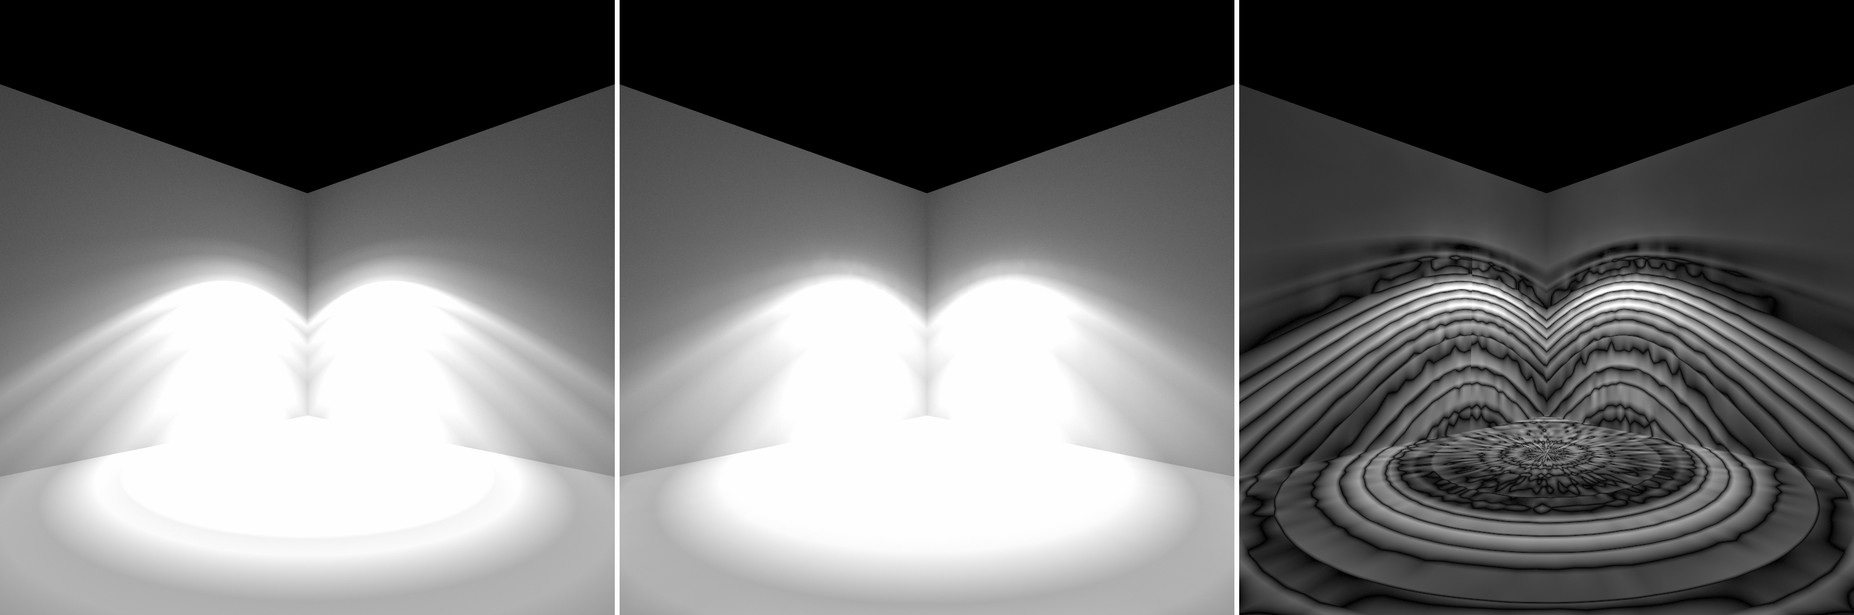
\includegraphics[width=0.86\textwidth]{lightrec_panel_point_228.jpg}\\[2pt]
    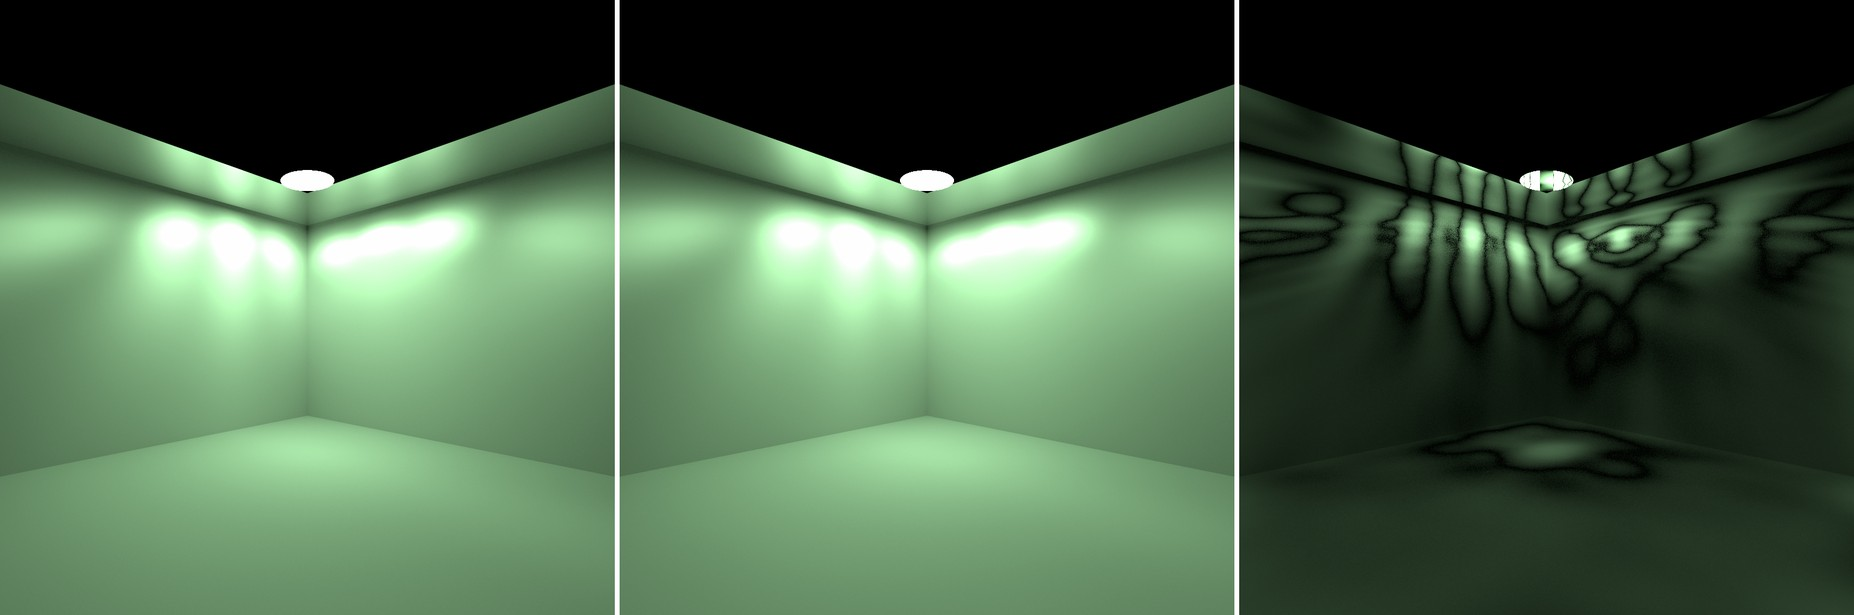
\includegraphics[width=0.86\textwidth]{lightrec_panel_disk_208.jpg}\\[2pt]
    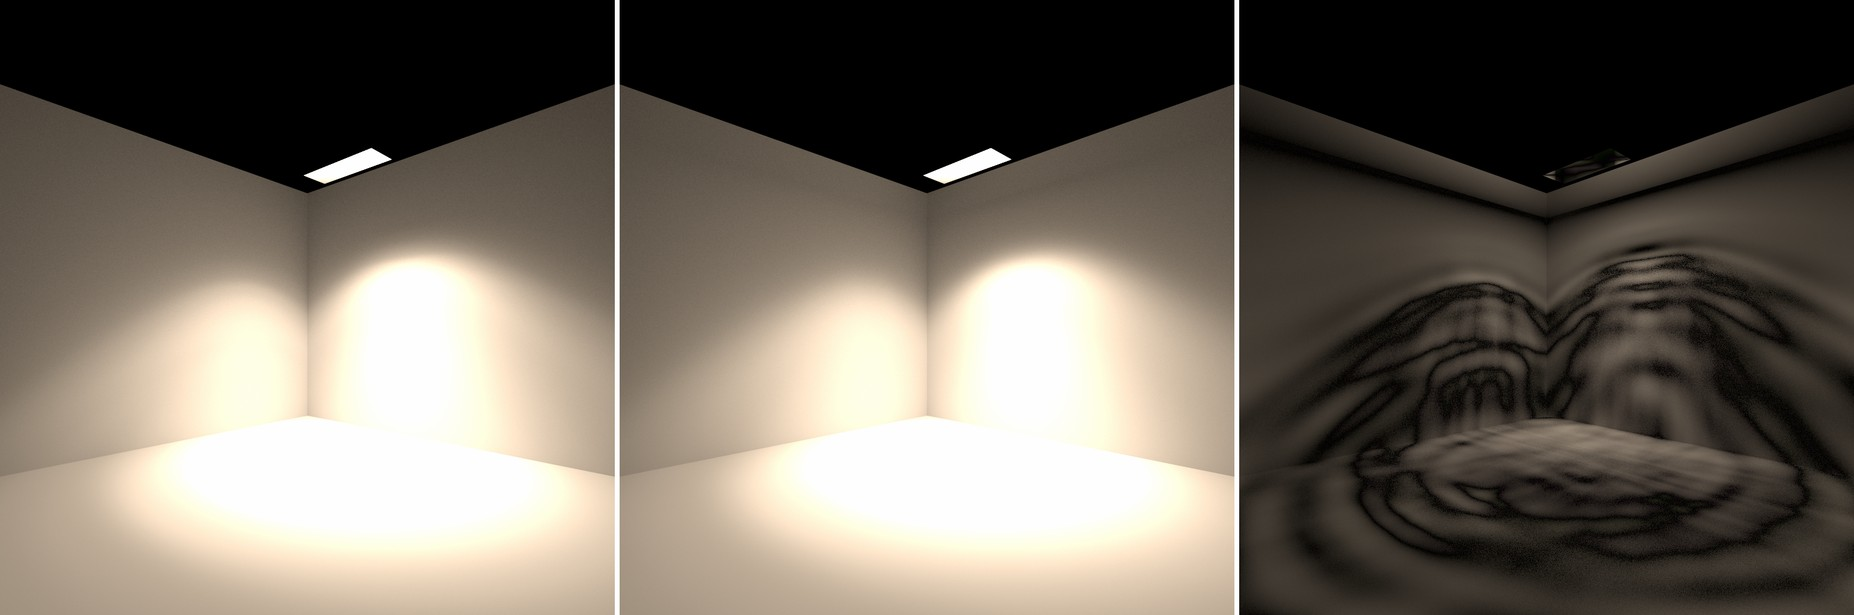
\includegraphics[width=0.86\textwidth]{lightrec_panel_rect_206.jpg}
    \caption{Примеры реконструкции: точечный источник (38.4~дБ), диск (43.8~дБ), прямоугольник (41.6~дБ). Слева направо: эталонное изображение, изображение сцены с восстановленным источником, модуль разности, увеличенный в 4 раза.}
    \label{fig:ies-panels}
\end{figure}

Следует отметить два свойства получаемого решения. Во-первых, по одному изображению наблюдаема только часть направлений излучения: в рассмотренных сценах от 45 до 51\% узлов таблицы не влияют на изображение, так как свет в этих направлениях не попадает на видимые поверхности; в выходном файле таким узлам присвоено нулевое значение. Во-вторых, для площадных источников освещённость сцены является свёрткой диаграммы направленности с формой источника, поэтому мелкие детали диаграммы восстанавливаются сглаженными. В обоих случаях восстановленный источник наблюдаемо эквивалентен исходному для данной сцены и камеры, что и отражает метрика PSNR, но его таблица не обязана совпадать с исходной.

\section{Сравнение с Mitsuba 3}

\subsection{Постановка сравнения}

Mitsuba~3 не содержит источников с гониометрической диаграммой, поэтому сравнение проводилось на источнике, который поддерживают обе системы: прямоугольном ламбертовском источнике с пространственно неоднородной яркостью, заданной RGB-текстурой $16\times16$ (768 неизвестных). В терминах главы~5 это текстурная модель с фиксированным углом половинной мощности $\theta=60^\circ$. Геометрия сцены, камера, разрешение изображения ($1024\times1024$) и глубина путей в обеих системах одинаковы; истинная текстура содержит три ярких пятна на более тёмном фоне и плавное изменение цвета.

Каждая система восстанавливает текстуру по эталонному изображению, рассчитанному ею самой с 2048 лучами на пиксель. Сравнивались следующие варианты.
\begin{itemize}
    \item \emph{Mitsuba~3, PRB.} На каждом шаге изображение рассчитывается заново с 16 лучами на пиксель и дифференцируется методом PRB; текстура обновляется методом Adam с проекцией на неотрицательные значения, функция потерь --- средний модуль разности. Использовались версии для графического (\texttt{cuda\_ad\_rgb}) и центрального (\texttt{llvm\_ad\_rgb}) процессоров, Mitsuba~3.9.1.
    \item \emph{Предложенный метод, Adam по кэшу.} Кэш световых путей строится один раз (16 лучей на пиксель, 4 выборки источника в первой вершине пути), после чего выполняются шаги метода Adam с аналитическим градиентом.
    \item \emph{Предложенный метод, решение методом наименьших квадратов (МНК).} Поскольку изображение линейно по яркости текстуры, по тому же кэшу за один проход накапливается система нормальных уравнений, которая решается разложением Холецкого отдельно для каждого цветового канала.
\end{itemize}

Чтобы исключить влияние различий между системами расчёта освещённости, результаты всех вариантов оценивались одинаково: восстановленная текстура подставлялась в сцену Mitsuba, изображение рассчитывалось с 512 лучами на пиксель и сравнивалось с эталоном Mitsuba. Истинная текстура при такой оценке даёт PSNR 46.47~дБ (в линейном HDR-представлении --- 75.5~дБ); это предел, определяемый шумом Монте--Карло контрольных изображений. Дополнительно вычислялась относительная ошибка текстуры --- сумма модулей отклонений от истинной текстуры, делённая на сумму её значений.

\subsection{Результаты}

\begin{table}[htbp]
    \centering
    \small
    \setlength{\tabcolsep}{4pt}
    \begin{tabular}{lccccc}
        \toprule
        Метод & \makecell{Время,\\с} & \makecell{Шаг,\\мс} & \makecell{PSNR,\\дБ} & \makecell{PSNR (HDR),\\дБ} & \makecell{Ошибка\\текстуры, \%} \\
        \midrule[\heavyrulewidth]
        Предложенный, МНК (CPU)  & \textbf{2.2}  & ---  & 46.47 & \textbf{75.3} & \textbf{0.07} \\
        Mitsuba 3 (GPU)             & 3.7           & 39   & 46.47 & 69.5 & 0.60 \\
        Mitsuba 3 (GPU), 300 шагов  & 11.7          & 39   & 46.47 & 70.9 & 0.52 \\
        Mitsuba 3 (CPU)             & 28.5          & 358  & ---$^{*}$ & 68.1 & 0.64 \\
        Предложенный, Adam (CPU) & 17.7          & 160  & 44.50 & 49.0 & 1.9 \\
        \midrule
        Истинная текстура                & ---           & ---  & 46.47 & 75.5 & 0 \\
        \bottomrule
    \end{tabular}
    \caption{Реконструкция текстуры яркости $16\times16$ прямоугольного источника по изображению $1024\times1024$. Время предложенного метода включает загрузку сцены и изображения и построение кэша (1.3~с); время Mitsuba~3 включает только шаги оптимизации. Для вариантов Mitsuba~3 в строках без указания числа шагов приведён первый контрольный момент, в который достигнут предельный PSNR (80 шагов). $^{*}$Контрольные изображения этого запуска рассчитаны с меньшим числом лучей, и его PSNR несопоставим с остальными строками.}
    \label{tab:mitsuba}
\end{table}

\begin{figure}[htbp]
    \centering
    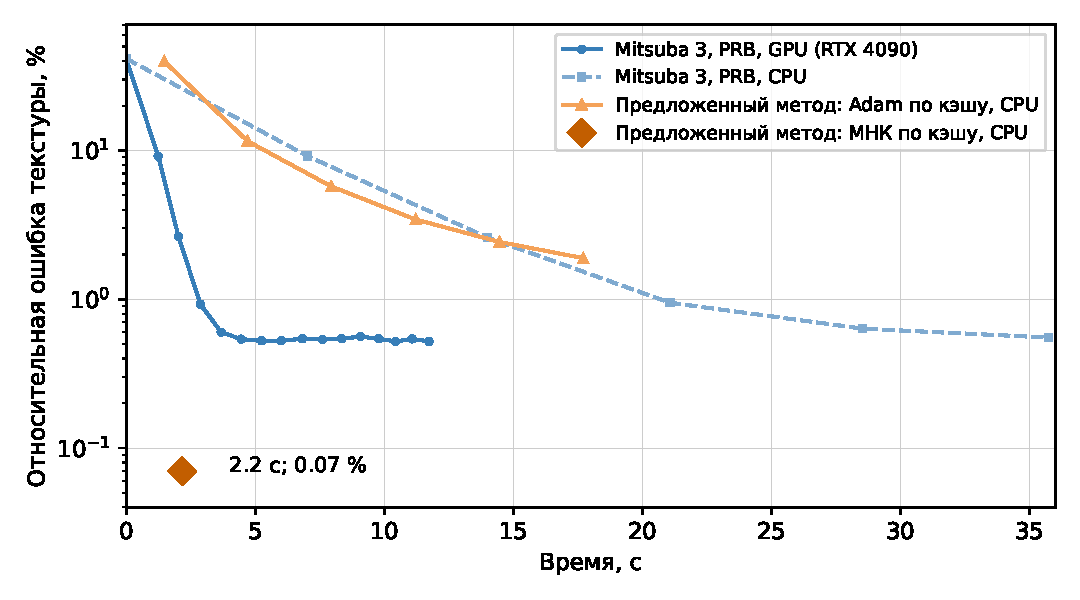
\includegraphics[width=0.82\textwidth]{lightrec_mitsuba_time.pdf}
    \caption{Относительная ошибка восстановленной текстуры в зависимости от времени реконструкции.}
    \label{fig:mitsuba-time}
\end{figure}

Результаты приведены в таблице~\ref{tab:mitsuba} и на рисунке~\ref{fig:mitsuba-time}. Решение методом наименьших квадратов по кэшу световых путей достигает предельного для данной оценки PSNR 46.47~дБ за 2.2~с. Mitsuba~3 на графическом процессоре RTX~4090 достигает того же значения PSNR за 3.7~с, то есть в 1.7 раза медленнее, а на том же центральном процессоре выходит на свою предельную точность (ошибка текстуры 0.6\%) за 21--28~с, то есть в 10--13 раз медленнее. При этом итоговая ошибка текстуры у предложенного метода в 7 раз меньше (0.07\% против 0.5\%): точность Mitsuba~3 ограничена шумом изображений, рассчитываемых на каждом шаге с 16 лучами на пиксель, и после 100 шагов перестаёт улучшаться.

Источник выигрыша --- не более быстрый шаг оптимизации, а структура задачи. Шаг метода Adam по кэшу на центральном процессоре (160~мс) в 2.2 раза быстрее шага Mitsuba~3 на том же процессоре (358~мс), но в 4 раза медленнее шага Mitsuba~3 на графическом процессоре (39~мс), и за 100 шагов этот вариант не сходится. Преимущество даёт то, что при фиксированной геометрии изображение линейно по параметрам излучения: кэш позволяет один раз вычислить эту линейную зависимость и решить задачу напрямую, тогда как система общего назначения заново трассирует и дифференцирует световые пути на каждом шаге.

Сравнение имеет следующие ограничения. Оно выполнено на одной сцене с простой геометрией и на источнике без диаграммы направленности; для источников с гониометрической диаграммой, которые Mitsuba~3 не поддерживает, сравнение времени не проводилось. Время Mitsuba~3 не включает загрузку сцены и компиляцию графа вычислений до первого шага. Замеры выполнены на графическом процессоре RTX~4090, более производительном, чем эталонное оборудование технического задания; на менее производительном графическом процессоре время Mitsuba~3 будет больше, а время предложенного метода от графического процессора не зависит.

\section{Соответствие требованиям технического задания}

Сводка результатов по требованиям технического задания к методу реконструкции освещения и к системе LightCadRenderCore приведена в таблице~\ref{tab:tz-light}.

\begin{table}[htbp]
    \centering
    \small
    \renewcommand{\arraystretch}{1.15}
    \begin{tabularx}{\textwidth}{>{\raggedright\arraybackslash}p{0.37\textwidth} X}
        \toprule
        \textbf{Требование} & \textbf{Результат} \\
        \midrule
        П.~4.1.17: PSNR изображения с восстановленными параметрами освещения относительно эталона не менее 25~дБ
            & 38.4--50.4~дБ на восьми сценах с точечным источником, диском и прямоугольником (таблица~\ref{tab:ies-results}) \\
        П.~4.1.18: время вычисления градиента не более 10 минут на кадр для одного шага оптимизации
            & 11--29~мс на шаг при изображении $1024\times1024$, центральный процессор AMD Ryzen~9 7950X (16 ядер) \\
        П.~4.1.19: время реконструкции в сравнении с аналогом при примерно одинаковом PSNR
            & Аналог --- Mitsuba~3 (PRB). При PSNR 46.47~дБ: 2.2~с против 3.7~с на графическом процессоре RTX~4090 и 21--28~с на центральном процессоре (таблица~\ref{tab:mitsuba}) \\
        П.~4.1.24: система LightCadRenderCore, время вычисления градиента не более 10 минут на кадр, входное изображение не менее $1024\times1024$
            & Приложение \texttt{lightcad} (раздел~\ref{sec:lightcad}); входное изображение $1024\times1024$, градиент 11--30~мс на шаг, полный цикл <<реконструкция --- расчёт изображения --- сравнение>> занимает менее минуты \\
        \bottomrule
    \end{tabularx}
    \caption{Соответствие результатов требованиям технического задания.}
    \label{tab:tz-light}
\end{table}

\endinput
